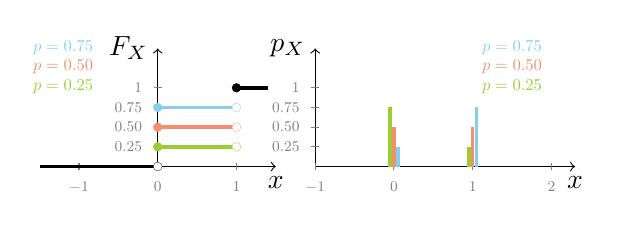
\begin{tikzpicture}
\begin{scope}
    % Axis
    \draw[->] (-1.5, 0) -- (1.5, 0) node[below]{$x$};
    \draw[->] (0, 0) -- (0, 1.5) node[left]{$F_X$};

    % Axis labels
    \foreach \x in {-1, ..., 1} {
        \draw [gray] (\x, 0.05) -- ++(0, -.1) ++(0, -.15) node [below, outer sep=0pt, inner sep=0pt, scale=0.6] {\small\(\x\)};}
    \foreach \y in {0.25, 0.50, 0.75, 1} {
        \draw [gray] (0.05, \y) -- ++(-.1, 0) ++(-.15, 0) node [left, outer sep=0pt, inner sep=0pt, scale=0.6] {\small\(\y\)};}

    % Definitions
    \def\pOne {0.25}
    \def\pTwo {0.50}
    \def\pThree {0.75}

    \def\firstColor {YellowGreen};
    \def\secondColor {Melon};
    \def\thirdColor {SkyBlue};
    
    % Legend
    \node [above, text=\firstColor,scale=0.6] at (-1.2,\pOne + 0.6) {$p = \pOne$};
    \node [above, text=\secondColor,scale=0.6] at (-1.2,\pTwo + 0.6) {$p = \pTwo$};
    \node [above, text=\thirdColor,scale=0.6] at (-1.2,\pThree + 0.6) {$p = \pThree$};
    
    % Function
    \draw[draw=black,line width=1.3pt] (-1.5,0) -- (0,0);
    \filldraw[draw=black,line width=0.1pt,fill=white] (0,0) circle[radius=1.6pt];

    \draw[draw=\firstColor,line width=1.3pt] (0,\pOne) -- (1,\pOne);
    \filldraw[draw=\firstColor,line width=0.1pt,fill=\firstColor] (0,\pOne) circle[radius=1.6pt];
    \filldraw[draw=\firstColor,line width=0.1pt,fill=white] (1,\pOne) circle[radius=1.6pt];

    \draw[draw=\secondColor,line width=1.3pt] (0,\pTwo) -- (1,\pTwo);
    \filldraw[draw=\secondColor,line width=0.1pt,fill=\secondColor] (0,\pTwo) circle[radius=1.6pt];
    \filldraw[draw=\secondColor,line width=0.1pt,fill=white] (1,\pTwo) circle[radius=1.6pt];

    \draw[draw=\thirdColor,line width=1.3pt] (0,\pThree) -- (1,\pThree);
    \filldraw[draw=\thirdColor,line width=0.1pt,fill=\thirdColor] (0,\pThree) circle[radius=1.6pt];
    \filldraw[draw=\thirdColor,line width=0.1pt,fill=white] (1,\pThree) circle[radius=1.6pt];
    
    \draw[draw=black,line width=1.3pt] (1,1) -- (1.4,1);
    \filldraw[draw=black,line width=0.1pt,fill=black] (1,1) circle[radius=1.6pt];
\end{scope}
\begin{scope}[xshift=3cm]
    % Axis
    \draw[->] (-1, 0) -- (2.3, 0) node[below]{$x$};
    \draw[->] (-1, 0) -- (-1, 1.5) node[left]{$p_X$};

    % Axis labels
    \foreach \x in {-1, ..., 2} {
        \draw [gray] (\x, 0.05) -- ++(0, -.1) ++(0, -.15) node [below, outer sep=0pt, inner sep=0pt, scale=0.6] {\small\(\x\)};}
    \foreach \y in {0.25, 0.50, 0.75, 1} {
        \draw [gray] (-0.95, \y) -- ++(-.1, 0) ++(-.15, 0) node [left, outer sep=0pt, inner sep=0pt, scale=0.6] {\small\(\y\)};}

    % Definitions
    \def\pOne {0.25}
    \def\pTwo {0.50}
    \def\pThree {0.75}

    \def\firstColor {YellowGreen};
    \def\secondColor {Melon};
    \def\thirdColor {SkyBlue};
    
    % Legend
    \node [above, text=\firstColor,scale=0.6] at (1.5,\pOne + 0.6) {$p = \pOne$};
    \node [above, text=\secondColor,scale=0.6] at (1.5,\pTwo + 0.6) {$p = \pTwo$};
    \node [above, text=\thirdColor,scale=0.6] at (1.5,\pThree + 0.6) {$p = \pThree$};
    
    % Function
    \draw[draw=\firstColor,line width=1.3pt] (-0.05,0) -- (-0.05,1-\pOne);
    \draw[draw=\secondColor,line width=1.3pt] (0,0) -- (0,1-\pTwo);
    \draw[draw=\thirdColor,line width=1.3pt] (0.05,0) -- (0.05,1-\pThree);    

    \draw[draw=\firstColor,line width=1.3pt] (0.95,0) -- (0.95,\pOne);    
    \draw[draw=\secondColor,line width=1.3pt] (1,0) -- (1,\pTwo);
    \draw[draw=\thirdColor,line width=1.3pt] (1.05,0) -- (1.05,\pThree);
\end{scope}
\end{tikzpicture}